\begin{frame}
    \frametitle{Material for Bundle Adjustment}
    \note{Extracted from Course by Cyrill Stachniss https://youtu.be/LKDLcKrWOIU?si=InRBlf5Nmf7mGM9H}
   
    \TODO{Make Bundle Adjustment slides}
   
    \begin{itemize}
    \item Cyrill Stachniss - The Basics about Bundle Adjustment
   
    Video: \url{https://youtu.be/sobyKHwgB0Y?si=EqmuOjWNwKBI9jqH}
   
    Slides: \url{https://www.ipb.uni-bonn.de/html/teaching/photo12-2021/2021-pho2-09-BA-part1.pptx.pdf}
    \item Cyrill Stachniss - The Numerics of Bundle Adjustment
   
    Video: \url{https://youtu.be/LKDLcKrWOIU?si=InRBlf5Nmf7mGM9H}
   
   Slides: \url{https://www.ipb.uni-bonn.de/html/teaching/photo12-2021/2021-pho2-10-BA-part2.pptx.pdf}
   \end{itemize}
   \end{frame}
   
   \begin{frame}
   \frametitle{Bundle Adjustment}
   \note{Information taken from https://youtu.be/BuRCJ2fegcc and https://youtu.be/mZBdPgBtrCM}
   
   Bundle Adjustment is a case in point
   
   \begin{itemize}
   \item 3D reconstruction based on images taken from different viewpoints
   \item Minimizes reprojection error onto the 2D image plane
   \item No notion of odometry (pose-pose) constraints)
   \item In general, it uses the Levenberg-Marquart minimization method.
   \item Developed in the field of photogrammetry. \footnote{Photogrammetry is the technique used to study and accurately define the shape, dimensions, and position in space of any object, essentially using measurements taken on one or more photographs of that object.} During the 1950s.
   \end{itemize}
   
   \end{frame}
   
   \begin{frame}
   \frametitle{Bundle Adjustment}
   
   \begin{figure}
   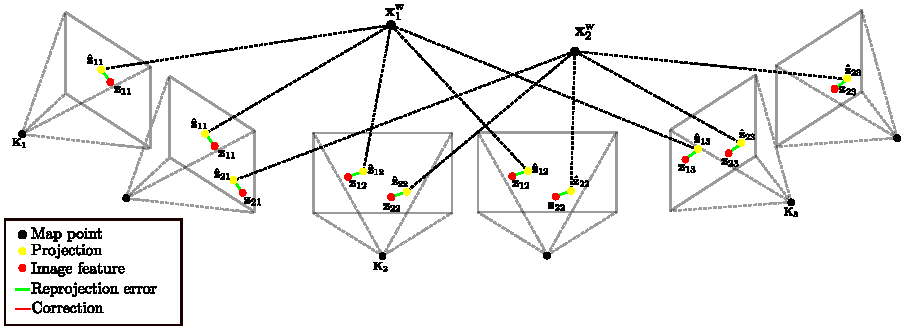
\includegraphics[width=\textwidth]{./images/ba_reprojection_error_before.pdf}
   \end{figure}
   
   \note{Example of adjusting 3 keyframes showing 2 points on the map.\\
   k1 - x1 stereo measurement\\
   k1 - x2 right measurement\\
   k2 - x1 stereo measurement\\
   k2 - x2 stereo measurement\\
   k3 - x1 measurement left\\
   k3 - x2 stereo measurement}
   
   \end{frame}
   
   \begin{frame}
   \frametitle{Bundle Adjustment}
   
   \begin{figure}
   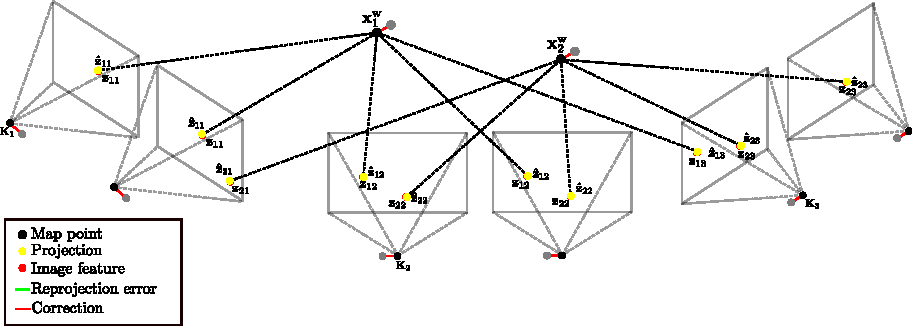
\includegraphics[width=\textwidth]{./images/ba_reprojection_error_after.pdf}
   \end{figure}
   
   \note{We adjust the keyframes and points!!!\\
   One error equation for each measurement (6 in total).\\
   We again take into account the rigid transformation between the left and right cameras for the right measurements.}
   
   \end{frame}
   
   \begin{frame}
   \frametitle{Bundle Adjustment}
   \note{Taken from Cyrill Stachniss https://youtu.be/LKDLcKrWOIU?si=InRBlf5Nmf7mGM9H}
   
   Least-squares approach to estimating camera poses and 3D points
   
   \textbf{Idea Key:}
   \begin{itemize}
   \item Start with an initial guess (\emph{initial guess})
   \item Project the estimated 3D points onto the estimated camera images
   \item Compare the locations of the 3D point projections with the measured 2D points
   \item Adjust to minimize error in the images
   \end{itemize}
   
   \end{frame}
   
   \begin{frame}
   \frametitle{Bundle Adjustment}
   \note{Taken from Cyrill Stachniss https://youtu.be/LKDLcKrWOIU?si=InRBlf5Nmf7mGM9H}
   
   \TODO{Add Bundle Adjustment content following Cyrill Stachniss's course}
   
\end{frame}